\chapter{Multivariate Regression Models for Time-Varying Graph Signals}

\lhead{Chapter 4. \emph{Multivariate Regression Models for Time-Varying Graph Signals}}

\label{chap:kgr_rnc_2d}

In this chapter, we focus on time-series regression models for graph signals. Specifically, our interest lies in the analysis of repeated measurements of a graph signal, where each sample is associated with a set of explanatory variables. The primary objective is to construct a predictive model capable of estimating these signals as a function of the aforementioned explanatory variables. Although regression has traditionally garnered less attention within the Graph Signal Processing (GSP) community compared to reconstruction, this framework holds significant relevance for numerous real-world applications. Consequently, it warrants further exploration and in-depth examination.

In the subsequent discussion, we emphasise two distinct data scenarios that may emerge within the context of graph signal regression. In the first scenario, the explanatory variables are exogenous or `global' with respect to the graph signals. In this setting, each graph signal $\y_t$ is accompanied by a feature vector $\x_t$, which is global in the sense that it is associated with the entire signal rather than a specific node. For example, consider predicting the quarterly earnings growth for a network of firms based on economic factors such as interest rates, inflation, and unemployment. A visual representation of the data present in such a scenario can be found in \cref{fig:KGR_diagram}.


\begin{figure}[ht]
    \centering
    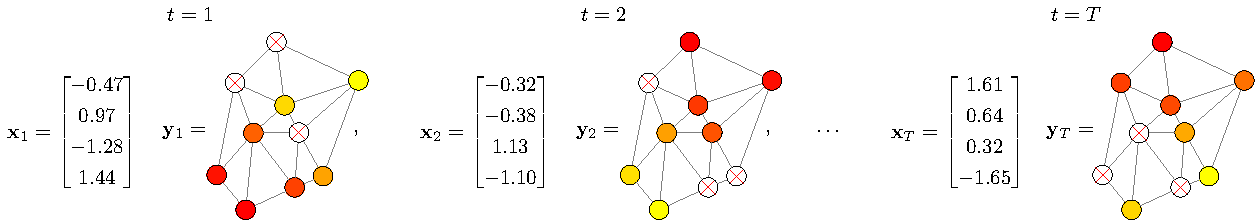
\includegraphics[width=\linewidth]{Figures/exogenous.pdf}
    \caption[Graph signal regression with exogenous variables]{A visual representation of a time-series graph signal regression problem with exogenous variables. Here, there are $T$ graph signals measured over a static graph, each with independent missing data (indicated in white with a red cross). Each signal $\y_t$ is accompanied by a unique vector of global explanatory variables $\x_t$. }
    \label{fig:KGR_diagram}
\end{figure}

In the second scenario under consideration, the explanatory variables are `local' to the nodes of the graph signal. This implies that for each graph signal $\y_t$, every node possesses an individual vector of explanatory variables $\x_{nt}$. For instance, consider a network of air quality monitoring stations with the objective of predicting the concentration of a specific airborne pollutant. Each station may simultaneously track various local factors, including temperature, pressure, precipitation, and so on. \Cref{fig:RNC_diagram} offers a visual depiction of the data encountered in this particular scenario.

\begin{figure}[ht]
    \centering
    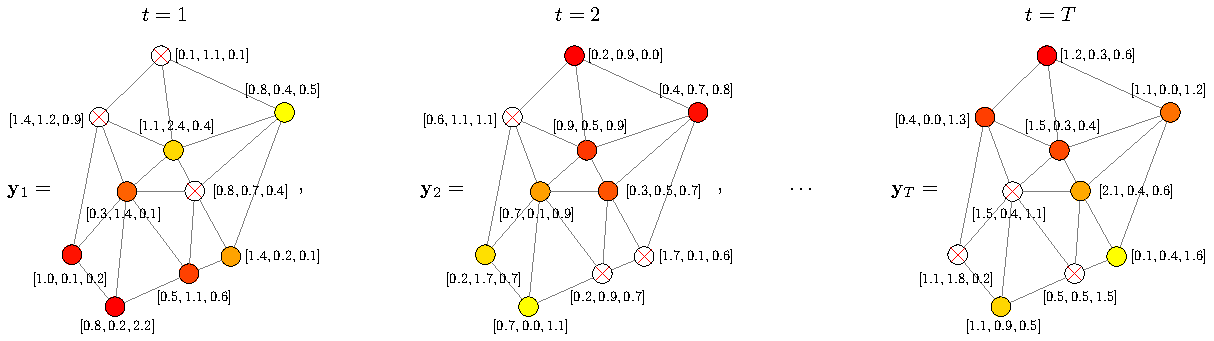
\includegraphics[width=\linewidth]{Figures/endogenous.pdf}
    \caption[Graph signal regression with local variables]{A visual representation of a time-series graph signal regression problem with local explanatory variables. As before, there are $T$ graph signals measured over a static graph, each with independent missing data (indicated in white with a red cross). In this case, each signal $\y_t$ has a vector of explanatory variables $\x_{nt}$ for every node in the signal. }
    \label{fig:RNC_diagram}
\end{figure}
  
The core goal of this chapter is to derive some useful extensions to existing methods for graph signal regression in both the local and global variable context. In the case of exogenous explanatory variables, we focus on Kernel Graph Regression (KGR) \citep{Venkitaraman2019,Elias2022} and the closely related topic of Gaussian Processes over Graphs (GPoG) \citep{Venkitaraman2020}. A notable issue in practice with existing KGR-type models is the assumption that the input signals $\y_t$ are always fully observed, meaning there is no missing data. As discussed in \cref{chap:gsr_2d}, a prevalent characteristic of graph signals in real-world applications is the high occurrence of missing data. This situation forces the end user to either eliminate entire rows (i.e., the complete time series for a specific node) if any elements in the series are not recorded, which may result in the loss of valuable topological information, or alternatively employ interpolation methods, which could prove inadequate for extended strings of missing data. Our proposed model accommodates fully general patterns of missing data in the input signals, enabling users to optimally utilise all available data.

For the scenario involving local explanatory variables, we enhance a model known as Regression with Network Cohesion (RNC) \citep{Li2019,Le2022} by incorporating several beneficial extensions. Specifically, the original RNC model was designed for a single graph signal rather than multiple repeated samples. Moreover, the original specification did not account for the presence of missing data. Consequently, we advance the model in at least two significant directions.

\section{Kernel Graph Regression with Unrestricted Missing Data Patterns}

\label{sec:kgr_mdp}

\subsection{Model description}

\label{sec:kgr_model_desc}

Consider a sequence of $T$ real-valued graph signals measured over a static $N$-node graph, for which an arbitrary subset of the elements of each signal may be missing, including potentially the entire signal at certain time points. At each time $t$, there also exists a vector of variables $\x_t \in \R^M$ encompassing $M$ distinct explanatory features. Each graph signal may have unique and arbitrary missing data, as indicated by a binary vector where ones represent successfully collected data and zeros signify missing data. Any absent data in $\y_t$ should be filled with zeros. Hence, the input data for this problem can be concisely described as follows. 


\begin{equation*}
    \text{input data} = \Big\{ \; \X \in \R^{T \times M}, \;\; \Y \in \R^{N \times T}, \;\; \Ss \in \{0, 1\}^{N \times T} , \;\; \A \in \R^{NT \times NT} \; \Big\}
\end{equation*}


 In the following, we assume that the explanatory variables do not contain missing values. However, if any missing values are present, conventional methods such as those described in \cite{Little2019} can be employed to fill them. It should be noted that, with this model specification, there is no rigid distinction between in-sample and out-of-sample prediction. To indicate a particular value of $\x_t$ for which a comprehensive prediction should be generated, one can set the corresponding value of $\y_t = \s_t = \zero$. 

As in \cref{sec:problem_statement_2d}, the graph signals can be stacked together into a matrix $\Y$ of shape $(N \times T)$. Note that this in contrast to the typical shape found in multivariate regression, which is most commonly $(T \times N)$ with the index referring to each sample varying first, however, we adopt the opposite convention here for the reasons outlined \cref{sec:gsp_cpg}. 

Consider now a $P$-dimensional basis function representation of each explanatory vector $\x_t$, denoted as $\boldsymbol{\phi}(\x_t) \in \R^{P}$. 

\begin{equation}
    \boldsymbol{\phi}(\x_t) = 
    \begin{bmatrix}
        \phi_1(\x_t) & \phi_2(\x_t) & \dots & \phi_P(\x_t)
    \end{bmatrix}^\top
\end{equation}

Let us assume that each element of $\y_t$ can be modelled as a noisy linear combination of these basis functions, which may or may not have been observed. This is summarised in the following statistical model. 

\begin{equation}
    \y_t = \s_t \circ \big( \mspace{1mu} \W \boldsymbol{\phi}(\x_t) + \e_t \mspace{1mu} \big), \quad \for \; t = 1, 2, ..., T
\end{equation}

Here, $\W \in \R^{N \times P}$ represents the model coefficients defining the linear combination, and $\e_t \in \R^{N}$ is a vector of i.i.d. Gaussian noise with zero mean and unit variance. The basis function vectors can be horizontally stacked together to form a design matrix $\PHI$. 

\begin{equation}
    \PHI \in \R^{P \times T} = \begin{bmatrix} 
        \phi_1(\x_1) & \phi_1(\x_2) & \dots & \phi_1(\x_T) \\
        \phi_2(\x_1) & \phi_2(\x_2) & \dots & \phi_2(\x_T) \\
        \vdots & \vdots & \ddots & \vdots  \\
        \phi_P(\x_1) & \phi_P(\x_2) & \dots & \phi_P(\x_T) \\
    \end{bmatrix}
\end{equation}

Therefore, the statistical model can be written in matrix form as 


\begin{equation}
    \Y = \Ss \circ \big( \mspace{1mu} \W \PHI + \E \mspace{1mu} \big)
\end{equation}

where $\Ss \in \{0, 1\}^{N \times T}$ is the binary sensing matrix as defined in \cref{sec:problem_statement_2d}, which is also each $\s_t$ stacked horizontally, and $\E \in \R^{N \times T}$ is a matrix of i.i.d. Gaussian noise with zero mean and unit variance. This implies that the probability distribution for $\vecc{\Y} \, | \, \W$ is given by 

\begin{equation}
    \vecc{\Y} \, | \, \W \sim \mathcal{N}\big( \vecc{\Ss \circ (\W \PHI)}, \; \I_{NT} \, \big)
\end{equation}

To determine the posterior distribution of the model coefficients $\W$, it is necessary to specify a prior that reflects the assumption that predicted signals are expected to be smooth with respect to the graph's topology. We assert that an appropriate prior for $\W$ is given by

\begin{equation}
\label{eq:W_prior}
\vecc{\W} \sim \mathcal{N}\left(\zero, \; \gamma^{-1} \I_P \otimes \HH_N^{2}\right)
\end{equation}

Here, $\HH_N \in \R^{N}$ represents a graph filter constructed in accordance with one of the univariate filter functions defined in \cref{tab:iso_filters}, while $\gamma$ serves as a hyperparameter denoting the prior precision. The rationale for this prior, as explicated in \cite{Venkitaraman2020}, is as follows. Consider a random graph signal formulated as $\W \boldsymbol{\phi}$, where both $\W$ and $\boldsymbol{\phi}$ have Gaussian i.i.d. entries with zero mean and unit variance. The probability distribution of their product will also be an i.i.d. multivariate Gaussian with zero mean. By applying a graph filter $\HH_N$ to smooth this signal, the resulting signal will exhibit the same probability distribution as $\W \boldsymbol{\phi}$, assuming $\W$ was drawn from the distribution specified in \cref{eq:W_prior}. Consequently, this prior serves to enhance the likelihood of smooth signals.


% https://stats.stackexchange.com/questions/28229/variance-of-the-product-of-a-random-matrix-and-a-random-vector

Consider now a transformed variable $\F$ defined by $\F = \W \PHI$. Given that $\W$ has a prior distribution given in \cref{eq:W_prior}, we can ask what the implied prior for $\F \, | \, \PHI$ is. Clearly, since the expected value of $\W$ is zero for all entries, the expected value of $\F$ should also be zero for all entries regardless of the value of $\PHI$. The covariance of $\F$ can also be computed easily. 

\begin{align*}
    \text{Cov}\big[\vecc{\F}\big] &= \text{Cov}\big[\vecc{\W \PHI}\big] \\[0.1cm]
    &= \text{Cov}\left[\big(\PHI^\top \otimes \I\big) \, \vecc{\W}\right] \\[0.1cm]
    &= \big(\PHI^\top \otimes \I\big) \, \text{Cov}\big[\vecc{\W}\big] \, \big(\PHI \otimes \I\big) \\[0.2cm]
    &= \gamma^{-1}  \big(\PHI^\top \otimes \I\big) \, \big(\I \otimes \HH_N^{2} \big) \, \big(\PHI \otimes \I\big) \\[0.2cm]
    &= \gamma^{-1} \big( \PHI^\top \PHI \big) \otimes \HH_N^2
\end{align*}

Therefore, we can rewrite the model in terms of the new transformed variable as follows. 

\begin{equation}
    \vecc{\Y} \, | \, \F \sim \mathcal{N}\big(\, \vecc{\Ss \circ \F}, \, \I_{NT} \, \big)
\end{equation}

\begin{equation}
    \label{eq:F_prior2}
    \vecc{\F} \sim \mathcal{N}\Big(\zero, \; \gamma^{-1} \big(\PHI^\top \PHI \big) \otimes \HH_N^{2}\Big)
\end{equation}


The final step to convert this into a non-parametric regression model is to apply the `kernel-trick' \citep{Scholkopf2018}. Consider the PSD matrix $\PHI^\top \PHI$. Entry $(i, j)$ will be the inner product between the basis function expansion of $\x_i$ and $\x_j$. 

\begin{equation}
    \PHI^\top \PHI \in \R^{T \times T} = 
    \begin{bmatrix} 
        \boldsymbol{\phi}(\x_1)^\top\boldsymbol{\phi}(\x_1) & \boldsymbol{\phi}(\x_1)^\top\boldsymbol{\phi}(\x_2) & \dots & \boldsymbol{\phi}(\x_1)^\top\boldsymbol{\phi}(\x_T) \\
        \boldsymbol{\phi}(\x_2)^\top\boldsymbol{\phi}(\x_1) & \boldsymbol{\phi}(\x_2)^\top\boldsymbol{\phi}(\x_2) & \dots & \boldsymbol{\phi}(\x_2)^\top\boldsymbol{\phi}(\x_T) \\
        \vdots & \vdots & \ddots & \vdots  \\
        \boldsymbol{\phi}(\x_T)^\top\boldsymbol{\phi}(\x_1) & \boldsymbol{\phi}(\x_T)^\top\boldsymbol{\phi}(\x_2) & \dots & \boldsymbol{\phi}(\x_T)^\top\boldsymbol{\phi}(\x_T) \\
    \end{bmatrix}
\end{equation}

The trick is to characterise each inner product in terms of a predefined function such that $\boldsymbol{\phi}(\x_i)^\top\boldsymbol{\phi}(\x_j) = \kappa(\x_i, \x_j)$. This means that instead of mapping the explanatory variables via $\boldsymbol{\phi}$ and computing the inner product directly, it is done in a single operation, leaving the mapping implicit. This means we can replace the matrix $\PHI^\top \PHI$ with a so-called kernel (or \textit{Gram}) matrix $\K \in \R^{T \times T}$, which has entries defined by 

\begin{equation}
    \label{eq:kernel_matrix}
    \K_{ij} = \kappa(\x_i, \x_j)
\end{equation}

where $\kappa(\cdot, \cdot)$ is any valid Mercer kernel \citep{Rasmussen2005}. A common example is the Gaussian kernel given below. 

\begin{equation}
    \label{eq:gaussian_kernel}
    \kappa(\x_i, \x_j) = \exp\left(-\frac{|| \x_i - \x_j ||^2}{2 \sigma^2}\right)
\end{equation}

Therefore, the prior distribution over $\F$ is given in terms of $\K$ by 

\begin{equation}
    \label{eq:F_prior3}
    \vecc{\F} \sim \mathcal{N}\Big(\zero, \; \gamma^{-1} \K \otimes \HH_N^{2}\Big)
\end{equation}

In a similar manner to \cref{sec:problem_statement_2d}, the posterior distribution for $\F | \Y$ is given by 

\begin{equation}
    \label{eq:F_post_kgr}
    \vecc{\F} \, | \, \Y \sim \mathcal{N}\left(\bar{\PP}^{-1}\vecc{\Y}, \; \bar{\PP}^{-1}\right)
\end{equation}

where $\bar{\PP}$ is the posterior precision matrix for $\vecc{\F}$, given by

\begin{equation}
    \label{eq:P_post_kgr}
    \bar{\PP} = \D_\Ss + \gamma \K^{-1} \otimes \HH_N^{-2}
\end{equation}

As before, $\D_\Ss = \diag{\vecc{\Ss}}$. 

\subsection{Relation to graph signal reconstruction}

\label{sec:KGR_and_GSR}

Despite arising from a different set of modelling assumptions, Kernel Graph Regression as described in \cref{sec:kgr_model_desc} bares a stark mathematical resemblance to Graph Signal Reconstruction. The only key difference between the specification of these two models is that in GSR, the prior distribution over $\vecc{\F}$ has covariance $\HH^2$ [see \cref{eq:F_prior}], and in KGR it has covariance $\K \otimes \HH_N^2$ [see \cref{eq:F_prior3}]. Intuitively speaking, the prior used in the GSR model encodes the belief that the underlying graph signal should be smooth with respect to the topology of the 2D Cartesian product graph. On the other hand, the prior used in the KGR model encodes the belief that the predicted signal should be smooth with respect to the topology of the 1D graph and the explanatory variables, i.e. graph signals $\y_i$ and $\y_j$ are expected to be similar if the vectors $\x_i$ and $\x_j$ are similar. 


As a result of the differences in their respective priors, the posterior precision matrix for $\vecc{\F}$ is given by $\D_\Ss + \gamma \HH^{-2}$ in the case of GSR and $\D_\Ss + \gamma \K^{-1} \otimes \HH_N^{-2}$ in the case of KGR. In both cases, it is the sum of $\D_\Ss$ and a Hermitian matrix. To make this correspondence clearer, we can expand the second term of each expression in terms of its respective eigendecomposition. For GSR, this is

\begin{align*}
    \D_\Ss + \gamma \HH^{-2} &= \D_\Ss + \gamma \big(\U_T \otimes \U_N \big) \, \diag{\vecc{\G}}^{-2} \, \big(\U_T^\top \otimes \U_N^\top \big) \\
    &= \D_\Ss + \U \, \D_\G^{-2} \, \U^\top
\end{align*}

where $\U = \U_T \otimes \U_N $, and $\D_\G = \diag{\vecc{\G}}$. For KGR this is

\begin{align*}
    \D_\Ss + \gamma \K^{-1} \otimes \HH_N^{-2} &= \D_\Ss + \gamma \big(\V \otimes \U_N \big) \, \diag{\vecc{\bar{\G}}}^{-2} \, \big(\V^\top \otimes \U_N^\top \big) \\
    &= \D_\Ss + \bar{\U} \, \D_{\bar{\G}}^{-2} \, \bar{\U}^\top
\end{align*}

where $\K$ and $\HH_N$ have eigendecompositions given by 

\begin{equation}
    \K = \V \LAM_K \V^\top, \aand \HH_N = \U_N \; g\left(\LAM_N\right)  \U_N^\top
\end{equation}

with $\LAM_K = \diag{\left[\lambda^{(K)}_1, \; \lambda^{(K)}_2, \; \dots, \;\lambda^{(K)}_T \right]}$, $\bar{\U} = \V \otimes \U_N$ and $\D_{\bar{\G}} = \diag{\vecc{\bar{\G}}}$. $\bar{\G} \in \R^{N \times T}$ has elements given by

\begin{equation}
    \bar{\G}_{nt} = g\left(\lambda^{(N)}_n\right) \sqrt{\lambda^{(K)}_t} \quad \Longleftrightarrow \quad \D_{\bar{\G}} = \LAM_K^{1/2} \otimes g\left(\LAM_N\right) 
\end{equation}



Therefore, KGR is algebraically equivalent to GSR under the following change of variables:

$$
\U \rightarrow \bar{\U}, \aand \G \rightarrow \bar{\G}
$$

As such, the iterative algorithms developed in \cref{chap:gsr_2d} can be largely recycled with only minor modifications. However, it is important to bear in mind that the value of the maximum entry in $\G$ is one, whereas the maximum value in $\bar{\G}$ is $\sqrt{\rho(\K)}$. This has some implications for the SIM and CGM convergence rate, as explored in the following sections. 


 

\subsection{Solving for the posterior mean}

We now briefly restate the SIM and CGM algorithms to highlight the small changes necessary to accommodate KGR with arbitrary missing data. The goal is to solve the following linear system 

\begin{equation}
    \label{eq:lin_system_kgr}
    \vecc{\F} = \Big(\D_\Ss + \gamma \K^{-1} \otimes \HH_N^{-2}\Big)^{-1} \vecc{\Y}
\end{equation}

First, let us revisit the SIM. Recall that the strategy is to split the coefficient matrix into $\M - \N$, where $\M$ is easy to invert. In this case, we can put

\begin{equation}
    \M = \gamma \K^{-1} \otimes \HH_N^{-2} + \I_{NT}, \aand \N = \D_{\Ss'}.
\end{equation}

where, as before, $\D_{\Ss'} = \diag{\mathbf{1} - \vecc{\Ss}}$. Consider the matrix $\M^{-1}$.

\begin{align}
    \label{eq:M_inv_kgr}
    \M^{-1} &= \Big(\gamma \K^{-1} \otimes \HH_N^{-2} + \I_{NT}\Big)^{-1} \notag \\[0.15cm]
    &= \Big(\gamma \bar{\U} \, \D_{\bar{\G}}^{-2} \, \bar{\U}^\top + \I_{NT}\Big)^{-1} \notag \\[0.2cm]
    &= \Big(\bar{\U} \, \big( \gamma \D_{\bar{\G}}^{-2} + \I_{NT} \big) \, \bar{\U}^\top\Big)^{-1} \notag \\[0.25cm]
    &= \bar{\U} \, \big( \gamma \D_{\bar{\G}}^{-2} + \I_{NT} \big)^{-1} \, \bar{\U}^\top \notag \\[0.2cm]
    &= \bar{\U} \, \D_{\bar{\J}} \, \bar{\U}^\top 
\end{align}

where $\D_{\bar{\J}} = \diag{\vecc{\bar{\J}}}$, and $\bar{\J} \in \R^{N \times T}$ has entries given by 

\begin{equation}
    \label{eq:Jnt2}
    \bar{\J}_{nt} = \frac{\lambda^{(K)}_t g^2\big(\lambda_n^{(N)}\big)}{ \raisebox{-0.2cm} { $\lambda^{(K)}_t g^2\big(\lambda_n^{(N)}\big) + \gamma$ } } = \frac{\bar{\G}_{nt}^2}{ \raisebox{-0.15cm} {$\bar{\G}_{nt}^2 + \gamma$}}
\end{equation}

The SIM algorithm then proceeds in much the same way as described in \cref{sec:SIM}. As before, it is clear to see that convergence will be achieved, since the spectral radius of $\M^{-1}\N$ will surely be less than one for any positive $\gamma$. In this case, the update formula is given by 

\begin{align}
    \label{eq:update_sim_kgr}
    \F_{k+1} & = \U_N \, \big( \bar{\J}  \circ \big( \U_N^\top \, (\Ss' \circ \F_{k})\, \V \big) \big) \, \V^\top + \F_0 \\
    \label{eq:update_sim_kgr2}
    \text{with} \quad\quad\quad \F_0 & = \U_N \, \big( \bar{\J}  \circ \big( \U_N^\top \, \Y \, \V \big) \big) \, \V^\top 
\end{align}

Note that each update step can be performed with $O(N^2T + NT^2)$ multiplications. 

Next, let us return to the CGM. Recall that the strategy for solving the linear system in \cref{eq:lin_system_kgr} is to utilise a symmetric a preconditioner $\PSI$ such that the new system is given by 

\begin{equation}
    \Big(\bar{\PSI} ^\top  \big(\D_\Ss + \gamma \K^{-1} \otimes \HH_N^{-2} \big) \, \bar{\PSI}   \Big) \Big(\bar{\PSI} ^{-1}\, \vecc{ \F } \Big) = \bar{\PSI} ^\top \, \vecc{\Y},
\end{equation}

$\bar{\PSI} $ should be chosen such that new coefficient matrix $\bar{\PSI} ^\top \big(\D_\Ss + \gamma \K^{-1} \otimes \HH_N^{-2} \big) \, \bar{\PSI} $ has a reduced condition number. In the present case, we assert that an effective preconditioner is given by 

\begin{equation}
    \bar{\PSI} = \big(\V \otimes \U_N \big) \, \diag{\vecc{\bar{\G}}} = \bar{\U} \D_{\bar{\G}}.
\end{equation}

This preconditioner transforms the coefficient matrix into 

\begin{align*}
    \bar{\PSI} ^\top \big(\D_\Ss + \gamma \K^{-1} \otimes \HH_N^{-2} \big) \, \bar{\PSI}   &= \D_{\bar{\G}} \, \big(\V^\top \otimes \U_N^\top \big) \, \big(\D_\Ss + \gamma \K^{-1} \otimes \HH_N^{-2} \big) \,  \big(\V \otimes \U_N \big) \, \D_{\bar{\G}}   \\[0.1cm]
    &= \D_{\bar{\G}} \, \big(\V^\top \otimes \U_N^\top \big) \, \D_\Ss \, \big(\V \otimes \U_N \big) \, \D_{\bar{\G}} + \gamma \I \\[0.1cm]
    &= \D_{\bar{\G}} \, \bar{\U} \, \D_\Ss \, \bar{\U}^\top \, \D_{\bar{\G}} + \gamma \I 
\end{align*}

Note that we can efficiently compute the action of multiplying this preconditioned matrix onto an arbitrary vector $\vecc{\RR} \in \R^{NT}$ as follows. 

$$
\mat{\big(\D_{\bar{\G}} \, \bar{\U} \, \D_\Ss \, \bar{\U}^\top \, \D_{\bar{\G}} + \gamma \I  \big)\, \vecc{\RR}} = \gamma \RR + \bar{\G} \circ \left(\U_N^\top \Big( \Ss \circ \big(\U_N (\bar{\G} \circ \RR) \V^\top \big) \Big) \V\right) 
$$

As with the SIM, this action can be performed with $O(N^2T + NT^2)$ multiplications. 



\section{Regression with Network Cohesion}

\label{sec:rnc_mdp}

\subsection{Model description}

In this model, we consider a sequence of $T$ real-valued signals, which are regularly sampled over a static $N$-node graph, and may contain arbitrary missing values. As with KGR and GSR, this is represented using an $(N \times T)$ matrix $\Y$, with missing values set to zero and further clarified with the binary sensing matrix $\Ss \in \{0, 1\}^{N \times T}$ which holds zeros at entries where the corresponding element of $Y$ is missing data, and ones elsewhere. In this model each node, $n$, at each time instant, $t$, under consideration, has an associated length-$M$ vector of explanatory variables $\x_{nt} \in \R^{M}$. The objective is to make use of both the node-level explanatory variables and the network topology to estimate the missing values in the graph signal. A visual depiction of the data available in this kind of scenario is given in \cref{fig:RNC_diagram}. 

\begin{equation*}
    \text{input data} = \Big\{ \;\Xt \in \R^{N \times T \times M}, \;\; \Y \in \R^{N \times T}, \;\; \Ss \in \{0, 1\}^{N \times T}, \;\; \LL \in \R^{NT \times NT} \; \Big\}
\end{equation*}

Here, we have introduced the notation $\Xt$, which is an order-3 tensor, which has three independent axes signifying node number $n$, time instant $t$, and covariate number $m$, respectively. In the following sections, we index/slice this tensor of explanatory variables, $\Xt$, in various ways, therefore, it is beneficial to establish some notational standards for this purpose. In general, we adhere to the conventions outlined in \cite{Kolda2009}, which are also similar to those found in \cite{Kiers2000}. 

To refer to an individual element of an order-3 tensor (i.e. a scalar entry), we use the notation $\Xt_{ntm}$. The object generated by fixing two indices and letting a third vary (resulting in a vector) is referred to in this context as a fibre. Using tensor notation, the vector of covariates $\x_{nt} \in \R^{M}$, which exists at every node, at every time point, can alternatively be written as $\Xt_{nt:}$. A two-dimensional section of a tensor (i.e. a matrix), where two indices can vary and a single index is fixed, is known as a slice. For example, we could consider the slice given by a specific covariate measured across the whole graph, at every time instant, for which we would use the notation $\Xt_{::m}$. \Cref{fig:X_tensor_indexing} gives a visual representation of several ways of indexing/slicing an order-3 tensor. 


\begin{figure}[t]  
    \centering
    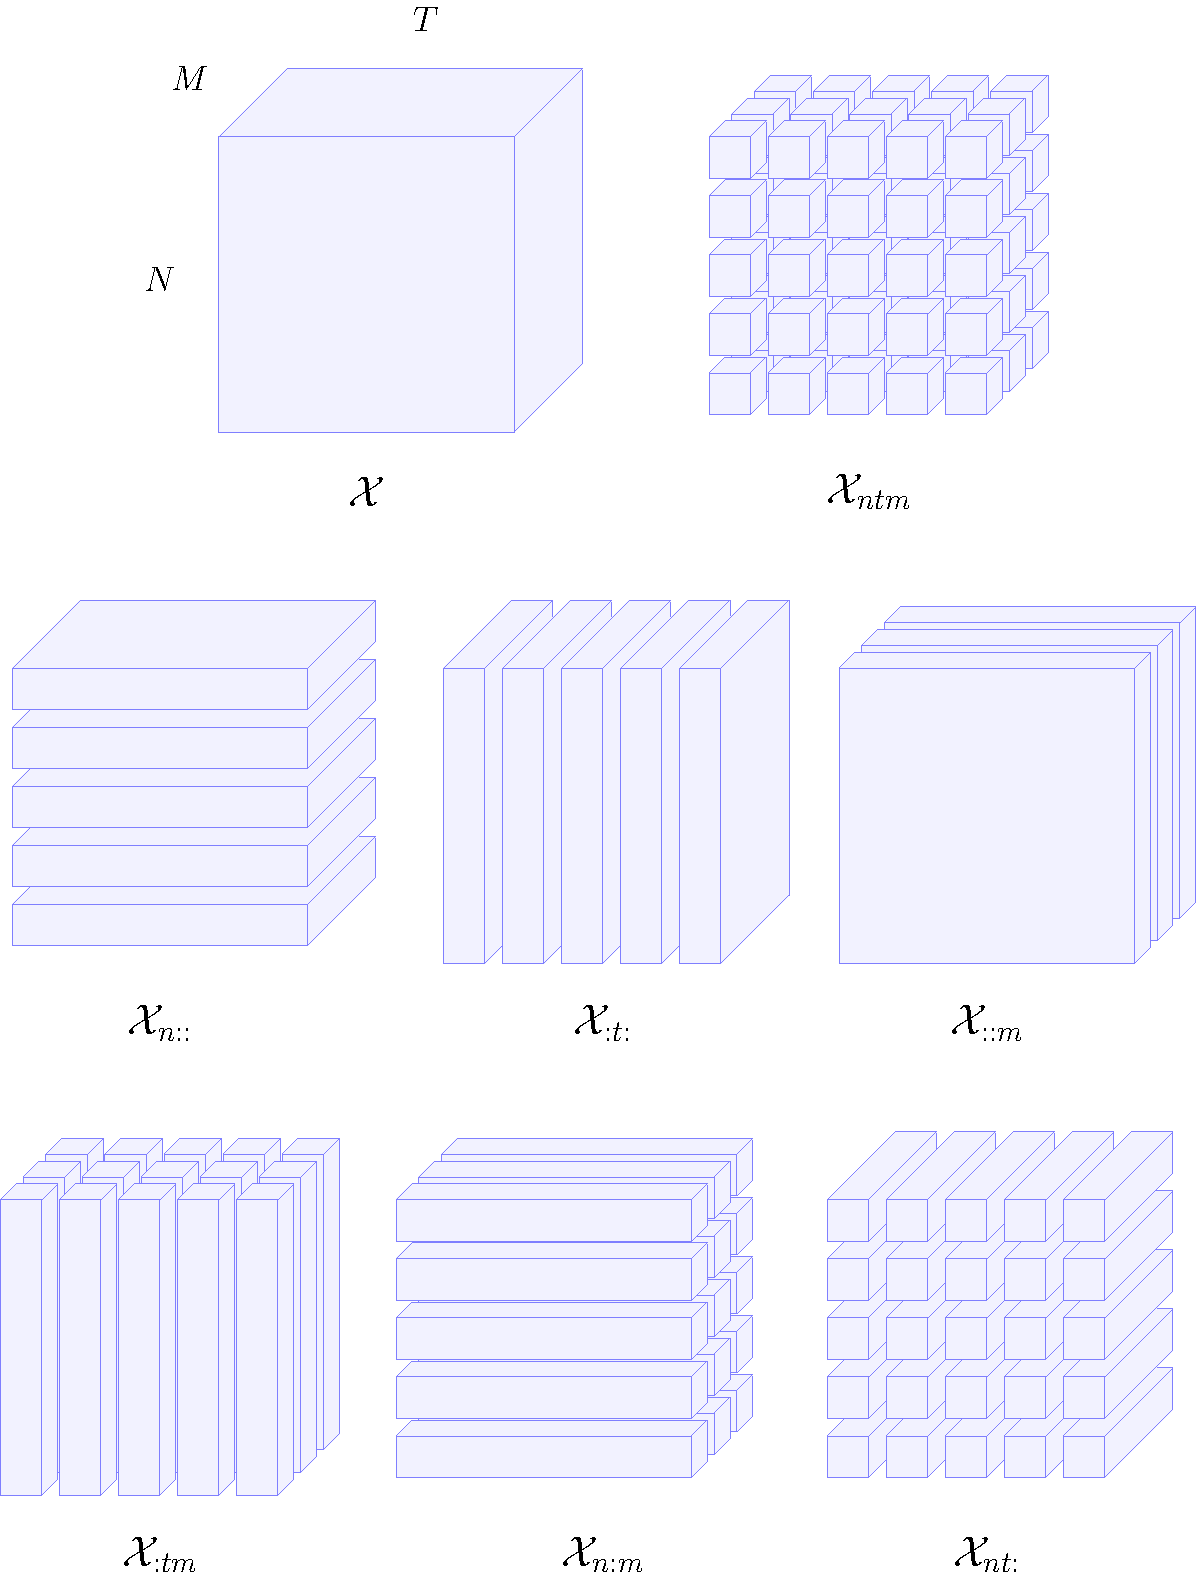
\includegraphics[width=0.6\linewidth]{Figures/X_tensor.pdf}
    \caption[Tensor indexing notation]{A visual representation of a several different ways of indexing into an order-3 tensor, with the corresponding notation indicated.}
    \label{fig:X_tensor_indexing}
\end{figure}


For the purposes of this section, we also define the special matrix $\X$, which is constructed by horizontally stacking the $M$ vectorized slices $\Xt_{::m}$, resulting in an object of shape $(NT \times M)$. 

\begin{equation}
    \label{eq:X_RNC}
    \X \in \R^{NT \times M} = \begin{bmatrix} \vecc{\Xt_{::1}} & \vecc{\Xt_{::2}} & \dots & \vecc{\Xt_{::M}} \end{bmatrix}    
\end{equation}

In this section we consider several extensions to a model known as Regression with Network Cohesion (RNC) \citep{Li2019}. In our version of the model, we assume that every element of the observed graph signal $\Y$ can be represented as the sum of an intercept term, a linear combination of the node-level covariates, and some Gaussian noise. However, the intercept term is flexible in the sense that each node/time can have a distinct value. To avoid underspecification, the model postulates that the intercepts are smooth with respect to the graph's topology. This is represented as follows. 

\begin{equation}
    \label{eq:rnc_stat_model_wc}
    \vecc{\Y} = \vecc{\Ss} \circ \big( \vecc{\C} + \X \w  + \vecc{\E} \big)
\end{equation}

In this context, $\C \in \R^{N \times T}$ represents the flexible intercept term, $\w \in \R^{M}$ the vector of regression coefficients, and $\E \in \R^{N \times T}$ a matrix of independent and identically distributed Gaussian noise with unit variance. The key assumption of the RNC model is that the intercept term $\C$ is smooth with respect to the topology of the entire $T-V$ Cartesian product graph. Furthermore, the above expression can be restated in terms of a single model coefficient vector $\thetaa$, by making use of the definition of $\X \in \R^{NT \times M}$ given in \cref{eq:X_RNC}, as follows.

\begin{equation}
    \label{eq:rnc_stat_model_theta}
    \vecc{\Y} = \vecc{\Ss} \circ \Big( \big[ \I_{NT} \;\; \X \big]\thetaa  + \vecc{\E} \Big)
\end{equation}

where $\big[ \I_{NT} \;\; \X \big] \in \R^{NT \times (NT + M)}$ is a block matrix consisting of the $(NT \times NT)$ identity matrix alongside $\X$, and $\thetaa$ is the block vector consisting of $\vecc{\C}$ stacked on top of $\w$, that is, 

\begin{equation}
    \thetaa \in \R^{NT + M} = \begin{bmatrix} \vecc{\C} \\ \w \end{bmatrix}
\end{equation}

Given \cref{eq:rnc_stat_model_theta}, we can write the probability distribution for $\Y \, | \, \thetaa$ as follows.  

\begin{equation}
    \label{eq:Y_given_theta_rnc}
    \vecc{\Y} \, | \, \thetaa \sim \mathcal{N}\left(\vecc{\Ss} \circ \Big( \big[ \I_{NT} \;\; \X \big]\thetaa \Big), \; \diag{\vecc{\Ss}}\right)
\end{equation}

In order to complete the specification of the Bayesian model, we need a prior distribution for $\thetaa$. In this case, we can independently combine both a graph-spectral prior for the $\vecc{\C}$ section and an L2 prior for the $\w$ section. This can be written as follows. 

\begin{equation}
    \label{eq:theta_prior}
    \thetaa \sim \mathcal{N}\left( \zero, \; \begin{bmatrix} \gamma^{-1} \HH^2 & \zero \\ \zero & \lambda^{-1} \I_M \end{bmatrix} \right)
\end{equation}

Here, $\HH \in \R^{NT \times NT}$ is a graph filter defined to act over the entire T-V product graph. This block matrix including $\HH$ and $\I_M$ both encodes the smoothness assumption for the flexible intercept term, and provides regularisation for the regression coefficients $\w$. Given this, the posterior distribution over $\thetaa$ is given by 

\begin{equation}
    \thetaa \, | \, \Y \sim \mathcal{N}\left(\widetilde{\PP}^{-1} \begin{bmatrix} \vecc{\Y} \\ \X^\top \vecc{\Y} \end{bmatrix}, \, \widetilde{\PP}^{-1}\right)
\end{equation}

where 

\begin{equation}
    \widetilde{\PP} \in \R^{(NT + M) \times (NT + M)}= 
    \begin{bmatrix}
     \D_\Ss + \gamma \HH^{-2} & \D_\Ss  \X \\
     \X^\top \D_\Ss & \X^\top \D_\Ss \X + \lambda \I_M   
    \end{bmatrix}
\end{equation}


A proof of this is given in \cref{the:RNC_post}. As before, $\D_\Ss = \diag{\vecc{\Ss}}$. 
    
\subsection{Solving for the posterior mean}

\label{sec:RNC_solving}

In the case of RNC, there is no simple or convenient way to reuse the SIM method to solve for the posterior mean. To see this, consider splitting the matrix $\widetilde{\PP}$ into $\M - \N$ where 

\begin{equation*}
    \M = 
    \begin{bmatrix}
        \I_{NT} + \gamma \HH^{-2} & \zero \\
        \zero & \lambda \I_M   
       \end{bmatrix}, 
       \aand \N = \begin{bmatrix}
        \D_{\Ss'} & -\D_\Ss  \X \\
        -\X^\top \D_\Ss & -\X^\top\D_\Ss \X 
       \end{bmatrix}
\end{equation*}

Recall that each iterative step in the SIM requires multiplication of a vector by $\M^{-1}\N$. Although $\M$ remains easy to invert, the spectral radius, $\rho(\M^{-1}\N)$ is no longer guaranteed to be less than one, resulting in a potential lack of convergence. This issue is not unique to a specific permutation of $\M$ and $\N$, but rather persists across multiple arrangements. 

On the other hand, we can find an effective preconditioner $\widetilde{\PSI}  \in \R^{(NT + M) \times (NT + M)}$ for use with the CGM, which transforms the linear system as follows. 

\begin{equation}
    \left( \widetilde{\PSI}^\top \begin{bmatrix}
        \D_\Ss + \gamma \HH^{-2} & \D_\Ss  \X \\
        \X^\top \D_\Ss & \X^\top \D_\Ss \X + \lambda \I_M   
       \end{bmatrix}  \widetilde{\PSI} \right) \left( \widetilde{\PSI}^{-1} \thetaa \right)   = \widetilde{\PSI}^\top \begin{bmatrix} \vecc{\Y} \\ \X^\top \vecc{\Y} \end{bmatrix}
\end{equation}


To obtain a suitable value for $\widetilde{\PSI}$, first let us define the eigendecomposition of $\X^\top\D_\Ss \X$. 

\begin{equation}
    \X^\top\D_\Ss \X = \U_M \LAM_M \U_M^\top
\end{equation}

Since $\X^\top\D_\Ss \X$ is positive semi-definite, $\U_M$ can be chosen to be orthonormal. Next, let us also introduce the diagonal matrix $\D_M$, which has the following definition 

\begin{equation}
    \D_M = \big(\LAM_M + \lambda \I_M \big)^{-1/2}
\end{equation}

We propose that an effective preconditioner is given by 

\begin{equation}
    \widetilde{\PSI} =  \begin{bmatrix}
        \U \D_\G & \zero \\
        \zero & \U_M \D_M 
    \end{bmatrix}
\end{equation}


where, as before, $\U = \U_T \otimes \U_N $. We choose this preconditioner because it transforms the block-diagonal elements of the original coefficient matrix $\widetilde{\PP}$ into matrices with eigenvalues bounded between $1 + \gamma$ and $\gamma$. In particular, the new coefficient matrix is given by

\begin{equation*}
    \widetilde{\PSI}^\top \widetilde{\PP}  \widetilde{\PSI} = 
       \begin{bmatrix}
        \D_\G \U^\top \D_\Ss \U \D_\G + \gamma \I_{NT}  &  \D_\G \U^\top \D_\Ss \X \U_M \D_M \\[0.1cm] 
        \D_M \U_M^\top \X^\top \D_\Ss \U \D_\G & \I_M
        \end{bmatrix}
\end{equation*}

Note that the upper left block can be multiplied onto a length $NT$ vector with complexity $O(N^2T + NT \log T)$, by leveraging the properties of the Kronecker product and making use of the Fast Cosine Transform (FCT). The upper right block of this matrix consists of $M$ length $NT$ column vectors, which can be computed with complexity $O(MN^2T + MNT \log T)$ and multiplied onto a length $M$ vector with complexity $O(NTM)$. This also applies to the lower left block, which is the transpose of the upper right, and can be multiplied onto a length $M$ vector in the same number of operations. Finally, the lower right block can be multiplied onto a length $M$ vector with $M$ operations. Therefore, the overall complexity of multiplying the entire matrix onto a vector of length $NT + M$ is $O(N^2T + NT \log T)$. 

\subsection{Discussion}

Limits as $\gamma, \lambda \rightarrow \infty$. 

\subsection{}

% Unfortunately, it is difficult to precisely quantify the spectrum of this block matrix. 



\section{Network regression with both global and local explanatory variables}

\label{sec:kgrnc}

In \cref{sec:kgr_mdp}, we introduced Kernel Graph Regression (KGR) with arbitrary missing values as a non-parametric regression technique, applicable for modelling scenarios where a series of graph signals need to be predicted based on exogenous or `global' explanatory variables. This concept is visually represented in \cref{fig:KGR_diagram}. On the other hand, Regression with Network Cohesion (RNC), discussed in \cref{sec:rnc_mdp}, is suitable for situations where `local' explanatory variables are associated with individual nodes over time, as depicted in \cref{fig:RNC_diagram}.

In certain cases, both global and local explanatory variables may coexist. For example, consider a network of businesses where firms are connected based on industry similarity or supply chain integration. In this scenario, the objective may be to predict quarterly revenue growth using variables affecting all firms, such as inflation and interest rates, while also considering firm-level local variables like employee turnover or debt ratio.

The input data in such a scenario can be summarised as follows

\begin{align*}
    \text{input data} &= \left\{\Xt \in \R^{N \times T \times M}, \; \X' \in \R^{T \times M'} \; \Y \in \R^{N \times T}, \; \Ss \in \{0, 1\}^{N \times T}, \; \A \in \R^{NT \times NT} \right\}
\end{align*}

Once again, $\Y$ is a sequence of partially observed graph signals and $\Ss$ is the corresponding binary sensing matrix  defining which values are missing. $\Xt$ represents the tensor of local explanatory variables, where each node at each time has an associated length-$M$ feature vector. In the example, this would represent the firm-level variables such as employee turnover and debt ratio. $\X'$ is the matrix of global explanatory variables, where the $t$-th row represents the global length-$M'$ feature vector at each time $t$. In this section we also continue to use the notation $\X$ (without the prime) to denote the matrix which is constructed by horizontally stacking the $M$ vectorized slices $\Xt_{::m}$, resulting in an object of shape $(NT \times M)$, as defined in \cref{eq:X_RNC}. 

Leveraging the methods developed for KGR and RNC in \cref{sec:kgr_mdp,sec:rnc_mdp}, we can naturally integrate both $\Xt$ and $\X'$ into the problem. The RNC model supposes that the observed graph signal is a noisy partial observation of a smooth underlying signal $\C$ added to a regularised linear combination of node-level covariates. Therefore, RNC combines aspects of graph signal reconstruction and ridge regression. As discussed in \cref{sec:KGR_and_GSR}, KGR can be understood as a small modification of the graph signal reconstruction problem, where the underlying signal $\F$ is instead assumed to be smooth with respect to both the 1D network and the explanatory variables, rather than a 2D Cartesian product graph. This involved altering the prior distribution over $\F$ to include the kernel matrix $\K$ which is a function of the global variables $\X'$, as defined in \cref{eq:kernel_matrix}. 

Similarly, we can modify the prior over the flexible intercept term $\C$ in the RNC model. Instead of using a prior covariance of $\gamma \HH^2$, we can employ a covariance matrix $\gamma \K \otimes \HH_N^2$, where $\K$ is the kernel matrix and $\HH_N$ is a graph filter acting upon the 1D network, as in the KGR model. Since the RNC model is defined in terms of the aggregate parameter vector $\thetaa$, we can adjust its prior distribution accordingly.

\begin{equation}
    \label{eq:theta_prior2}
    \hat{\thetaa} \sim \mathcal{N}\left( \zero, \; \begin{bmatrix} \gamma^{-1} \K \otimes \HH_N^2 & \zero \\ \zero & \lambda^{-1} \I_M \end{bmatrix} \right)
\end{equation}

Just as with KGR, this new model, which we refer to as Kernel Graph Regression with Network Cohesion (KG-RNC), is algebraically equivalent to the RNC model under the transformation 

$$
\U \rightarrow \bar{\U}, \aand \G \rightarrow \bar{\G}
$$

where $\K$ has an eigendecomposition $\V \LAM_K \V^\top$ and $\bar{\U}$ and $\bar{\G}$ are defined by

$$
\bar{\U} = \V \otimes \U_N, \aand     \bar{\G}_{nt} = g\left(\lambda^{(N)}_n\right) \sqrt{\lambda^{(K)}_t} \quad \rightarrow \quad \D_{\bar{\G}} = \LAM_K^{1/2} \otimes g\left(\LAM_N\right) 
$$

Given the prior for $\hat{\thetaa}$ in \cref{eq:theta_prior2}, and the likelihood which is identical to that of the RNC model given in \cref{eq:Y_given_theta_rnc}, the posterior distribution is given by 

\begin{equation}
    \hat{\thetaa} \, | \, \Y \sim \mathcal{N}\left(\hat{\PP}^{-1} \begin{bmatrix} \vecc{\Y} \\ \X^\top \vecc{\Y} \end{bmatrix}, \, \hat{\PP}^{-1}\right)
\end{equation}

where 

\begin{equation}
    \hat{\PP} \in \R^{(NT + M) \times (NT + M)}= 
    \begin{bmatrix}
     \D_\Ss + \gamma \K^{-1} \otimes \HH_N^{-2} & \D_\Ss  \X \\
     \X^\top \D_\Ss & \X^\top \D_\Ss \X + \lambda \I_M   
    \end{bmatrix}
\end{equation}

Once again, we can solve the linear system for the mean using the CGM, with a symmetric preconditioner $\hat{\PSI}$.  

\begin{equation}
    \left( \hat{\PSI}^\top \begin{bmatrix}
        \D_\Ss + \gamma \K^{-1} \otimes \HH_N^{-2} & \D_\Ss  \X \\
        \X^\top \D_\Ss & \X^\top \D_\Ss \X + \lambda \I_M   
       \end{bmatrix}  \hat{\PSI} \right) \left( \hat{\PSI}^{-1} \hat{\thetaa}\right)   = \hat{\PSI}^\top \begin{bmatrix} \vecc{\Y} \\ \X^\top \vecc{\Y} \end{bmatrix}
\end{equation}

where 

\begin{equation}
    \hat{\PSI} =  \begin{bmatrix}
        \bar{\U} \D_{\bar{\G}} & \zero \\
        \zero & \U_M \D_M 
    \end{bmatrix}
\end{equation}

The new preconditioned coefficient matrix in this case is given by 

\begin{equation*}
    \hat{\PSI}^\top \hat{\PP}  \hat{\PSI} = 
       \begin{bmatrix}
        \D_{\bar{\G}} \bar{\U}^\top \D_\Ss \bar{\U} \D_{\bar{\G}} + \gamma \I_{NT}  &  \D_{\bar{\G}} \bar{\U}^\top \D_\Ss \X \U_M \D_M \\[0.1cm] 
        \D_M \U_M^\top \X^\top \D_\Ss \bar{\U} \D_{\bar{\G}} & \I_M
        \end{bmatrix}
\end{equation*}

which can be efficiently multiplied onto a length $NT + M$ vector by leveraging the properties of the Kronecker product. Note that, in this case, the complexity of this multiplication is no longer $O(N^2T + NT \log T)$, but is now $O(N^2T + NT^2)$, since we cannot make use of the Fast Cosine Transform to multiply the matrix $\V \otimes \U$ onto a vector. 


\section{Network regression for pollutant monitoring}

In this section, we analyse the performance of the regression models developed in this chapter by applying them to an environmental modeling task. Our focus is on predicting the concentration of PM$_{2.5}$, a common airborne pollutant which consists of particulate matter with a diameter of 2.5 micrometers or less. We apply our models over a network of monitoring stations located in California, USA, using a dataset obtained from the U.S. Environmental Protection Agency's Air Data program. This program is responsible for generating daily readings of several airborne pollutants, including Ozone, Sulfur Dioxide (SO$_2$), Carbon Monoxide (CO), Nitrous Dioxide (NO$_2$), PM$_{2.5}$ and PM$_{10}$ at hundreds of locations across the country \citep{EPA2023}.  

In total, we consider $N=571$ monitoring stations across a period of $T=3957$ days from the 1$^\text{st}$ of January 2012 to the 30$^\text{th}$ of September 2022. Our method for graph construction was as follows. First, we took the latitude and longitude coordinates of each monitoring station and created a two-dimensional Voronoi diagram bounded by the California border \citep{Fortune1986}. This tessellated the state into 571 distinct regions; one per station. Next, we connected each pair of stations $i$ and $j$ if their respective Voronoi regions shared a boundary, and weight that connection by  $1 / (1 + kd_{ij})$, where $k$ is a scaling factor and $d_{ij}$ is their geodesic separation. This creates a sparse graph, which is visually represented in \cref{fig:cali_voronoi}. The total product graph used was then the Cartesian product between the size-$T$ path graph (i.e. $T$ nodes connected together in a chian representing time), and the cross-sectional network represented in \cref{fig:cali_voronoi}. 

\begin{figure}[ht]
    \centering
    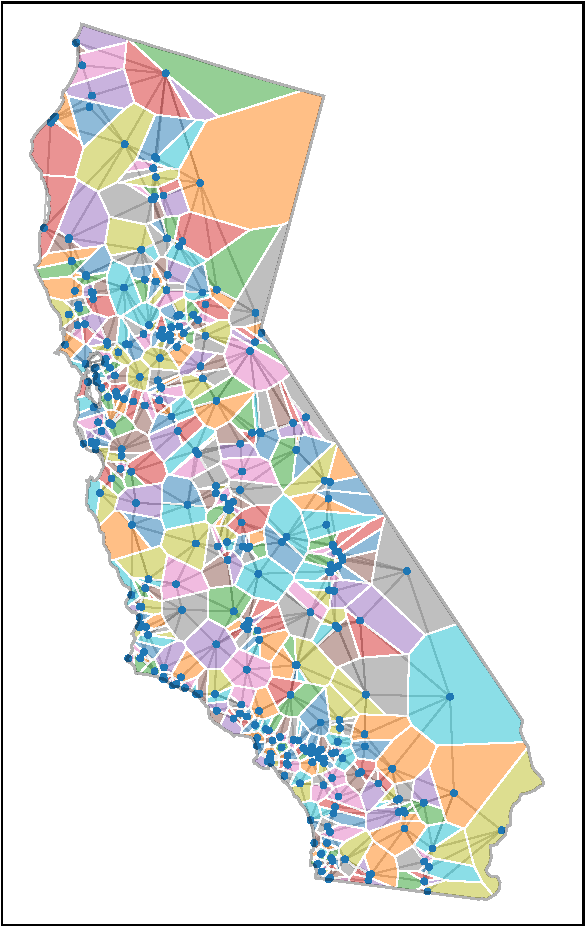
\includegraphics[width=0.6\linewidth]{Figures/cali_plot2.pdf}
    \caption[The network of monitoring stations created via Voronoi tessellation]{The network of monitoring stations, created via Voronoi tessellation. The geographic coordinates of the stations are used to create closed the regions, which are connected by a weighted edge to neighbouring regions. }
    \label{fig:cali_voronoi}
\end{figure}

In our experiments, we predicted $\log(1+c)$, where $c$ was the concentration of PM$_{2.5}$ in parts per million across the network using all three regression algorithms outlined in this chapter. In the case of Kernel Graph Regression, we used a set of global explanatory variables which were not associated with conditions at the individual monitoring stations, and for Regression with Network Cohesion, we used local explanatory variables that were associated with conditions at the individual monitoring stations. For KGR, we considered the number of active wildfires (which is known to be a strong contributor to PM$_{2.5}$ concentration \citep{Jaffe2020}) and meterological conditions across the state including temperature, pressure and humidity. In particular, for the wildfires, we calculated the number of acres actively burning on each day, within nine different regions using data from the CAL FIRE service from the Department of Forestry and Fire Protection \citep{CALFIRE2023}. For the meterological variables, we took readings also published by the Air Data program from locations across the state and took the first five principal components. 

For RNC, we used the other pollutants measured over the network, i.e. Ozone, SO$_2$, CO, NO$_2$, and PM$_{10}$. Since, in general, a considerable proportion of this data was missing, we first used Graph Signal Reconstruction. as described in \cref{chap:gsr_2d}, to interpolate the missing values. In addition, we used information local to each monitoring station such as land use and elevation. We also tested the KG-RNC framework outlined in \cref{sec:kgrnc} by combining both the local and global explanatory variables. Further information about the explanatory variables used is given in \cref{tab:features1,tab:features2}. 



\begin{table}[ht]
    \renewcommand{\arraystretch}{1.8}
    \centering
    \begin{tabular}{|l|p{11cm}|}
    \hline
    \multicolumn{2}{|c|}{\textbf{Global explanatory variables}} \\
    \hline
    \textbf{Variable} & \textbf{Description} \\
    \hline

    Time & A simple linear variable. \\

    Season & Two additional variables tracking season were created by taking the sin and cosine of $2 \pi t / 365$, where $t$ is the day of the year. \\

    Active wildfires & The original dataset comprised a list of wildfire events in California, containing information including the geographical coordinates, the start date, the end date and the total number of acres burned. Using the coordinates, we assigned each fire into one of nine regions. Then, by dividing the total acres burned by the incident duration, we calculated the average number of acres burning each day for each fire. By summing this for every region, we had an estimate of the total number of acres burning on each day for each region. \\

    Temperature & Using data from the Air Data program, we obtained readings for temperature at 90 locations across California. The readings were selected such that no missing data was present. Then, the first five principal components were taken. \\

    Pressure & As above, but for pressure. Readings from 48 locations were transformed into five PCA components. \\

    Humidity & As above, for humidity. Readings from 51 locations were transformed into five PCA components  \\
    \hline
    \end{tabular}
    \caption[Global explanatory variables used in the environmental modelling application]{The global explanatory variables used in this experiment. Each feature is not associated with any node in particular, but covaries with the graph signal over time. This resulted in a feature matrix $\X$ of shape $3957 \times 27$. All columns were normalised to have a mean of zero and standard deviation of one. }
    \label{tab:features1}
\end{table}

\begin{table}[ht]
    \renewcommand{\arraystretch}{1.8}
    \centering
    \begin{tabular}{|l|p{10.5cm}|}
    \hline
    \multicolumn{2}{|c|}{\textbf{Local explanatory variables}} \\
    \hline
    \textbf{Variable} & \textbf{Description} \\
    \hline
    Ozone & Ozone readings from the Air Data program were taken at all 571 monitoring stations. Where data was missing, graph signal reconstruction was used to interpolate the missing values. 72\% of the original data was missing. \\
    Sulfur Dioxide & As above. 95\% of the original data was missing.  \\
    Carbon Monoxide & As above. 89\% of the original data was missing.  \\
    Nitrous Dioxide & As above. 83\% of the original data was missing.  \\
    PM$_{10}$  & As above. 85\% of the original data was missing.  \\
    Elevation & The elevation of the station in meters. This variable remained constant over time \\
    Land use & Each monitoring station was had a land use flag, which was one of `Commercial', `Residential', `Agricultural', `Forest', `Industrial', `Desert', or `Military Reservation'. This was turned into a length-7 vector for each station using one-hot encoding which remained constant over time. \\
    Location setting & Each station also had a location flag, which was one of `Urban And Center City', `Suburban' or `Rural. In the same fashion as above, we created a one-hot encoding for each station, which remained constant over time. \\
    \hline
    \end{tabular}
    \caption[Local explanatory variables used in environmental modelling application]{The local explanatory variables used in this experiment. Each variable is associated with a monitoring station, and also varies over time. For elevation, land use and location setting which are fixed for each station, the values are simply repeated over time. This creates an explanatory tensor $\Xt$ of shape $571 \times 3957 \times 16$. }
    \label{tab:features2}
\end{table}
    
As a baseline approach, we also tested univariate and multivariate ridge regression using the local and global explanatory variables respectively. However, since multivariate ridge regression has no standard approach for the situation where values are missing from the multivariate targets, we first filled in these values according to the mean reading at each station. Where no readings were available at all at a particular station, we used the mean reading across time. 

In order to 

\cite{Cleland2020}. 

\begin{figure}[ht]
    \centering
    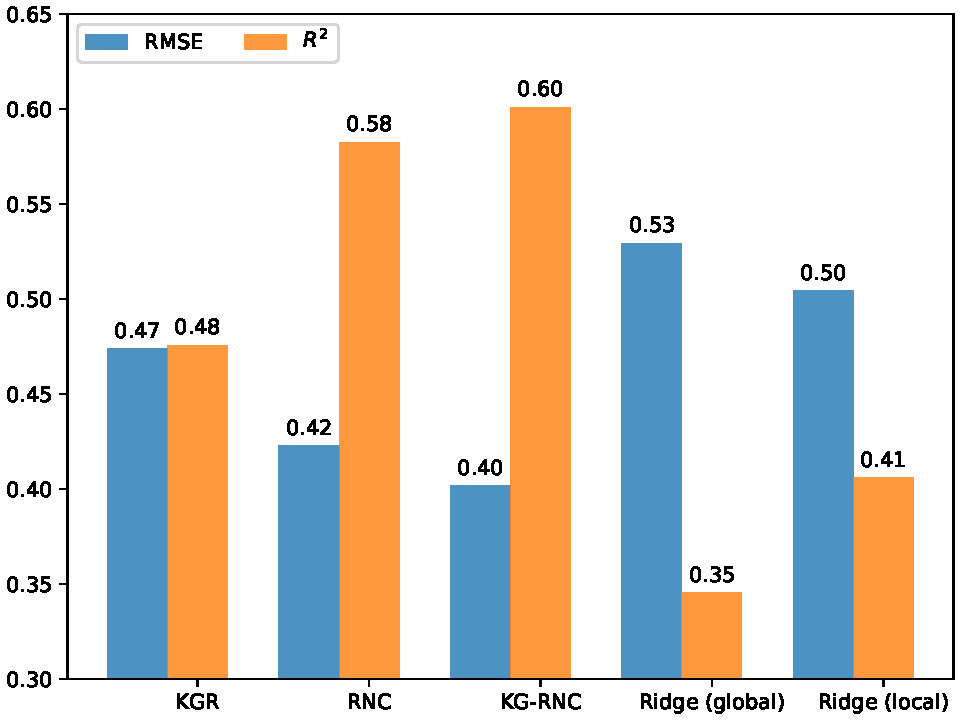
\includegraphics[width=0.85\linewidth]{Figures/regression_results.pdf}
    \caption[Graph signal regression with exogenous variables]{A visual representation of a time-series graph signal regression problem with exogenous variables. Here, there are $T$ graph signals measured over a static graph, each with independent missing data (indicated in white). Each signal $\y_t$ is accompanied by a unique vector of global explanatory variables $\x_t$. }
    \label{fig:regression_results}
\end{figure}